% !TEX encoding = UTF-8 Unicode
%!TEX root = thesis.tex
% !TEX spellcheck = en-US
%%=========================================
\section{Experiment 4}
In this experiment, the aim is to compare two different collections of audio features used in the similarity measure

Configuration A RMS, pitch and spectral centroid

Configuration B RMS, pitch, spectral centroid and bark bands

\subsection{Configuration}
\begin{minipage}{\linewidth}
\centering
\captionof{table}{Table Title TODO} \label{tab:exp4_configuration} 
\begin{tabular}{ C{2.5in} C{2.6in} }\toprule[1.5pt]
\bf Parameter & \bf Value \\
\midrule
  Number of generations & 500 \\
\midrule
  Fitness function & Local similarity \\
\midrule
  Target sound & Sine wave, 440 Hz \\
\midrule
  Input sound & White noise \\
\midrule
  Effect & Band-pass filter with up to 10x post gain \\
\midrule
  Audio features & \textbf{Configuration A}: RMS, pitch and spectral centroid \newline
  \textbf{Configuration B}: RMS, pitch, spectral centroid and 25 bark bands \\
\midrule
  Number of runs & 10 per configuration \\
\bottomrule[1.25pt]
\end {tabular}\par
\bigskip
Should be a caption TODO
\end{minipage}

\subsection{Evaluation}
Since fitness functions were different in these two configurations, the fitness values are not directly comparable. Instead, the results were evaluated by manually listening to the output sounds. In the first configuration, the results were fairly bad: All of the sounds were too noisy, and the author failed to perceive the tone. However, in terms of spectral centroid and amplitude, the sounds were a good match. In order to transform noise into a sine, the bandwidth of the band-pass filter has to be very narrow. A narrow filter would have lowered the overall amplitude of the sound. This would have been deemed bad by the fitness function, hence the genetic algorithm did not effectively explore that area in the solution space. Also, a narrow filter wouldn't have yielded any improvements in the similarity in spectral centroid and/or pitch. Therefore, the typical solution has a broad bandpass filter, albeit with an appropriate center frequency. See in figure \ref{fig:exp4_spectrum_plot} that the peak frequency of the typical output sound matches well the peak frequency of the target sound.

The results in the second configuration, were much better. The author could hear a clear tone in all 10 output sounds. There was still some noise in most sounds. The author believes that the solutions would have improved with more generations, because the fitness was typically still increasing towards the 500th (last) generation. One of the output sounds featured vibrato (varying pitch over time), due to a noisy input being mapped to the center frequency parameter. This could probably have been alleviated by adding the derivative of the pitch as a dimension in the fitness function, so the unwanted vibrato would be punished more severely by the fitness function.

\begin{figure}[h]
    \centering
    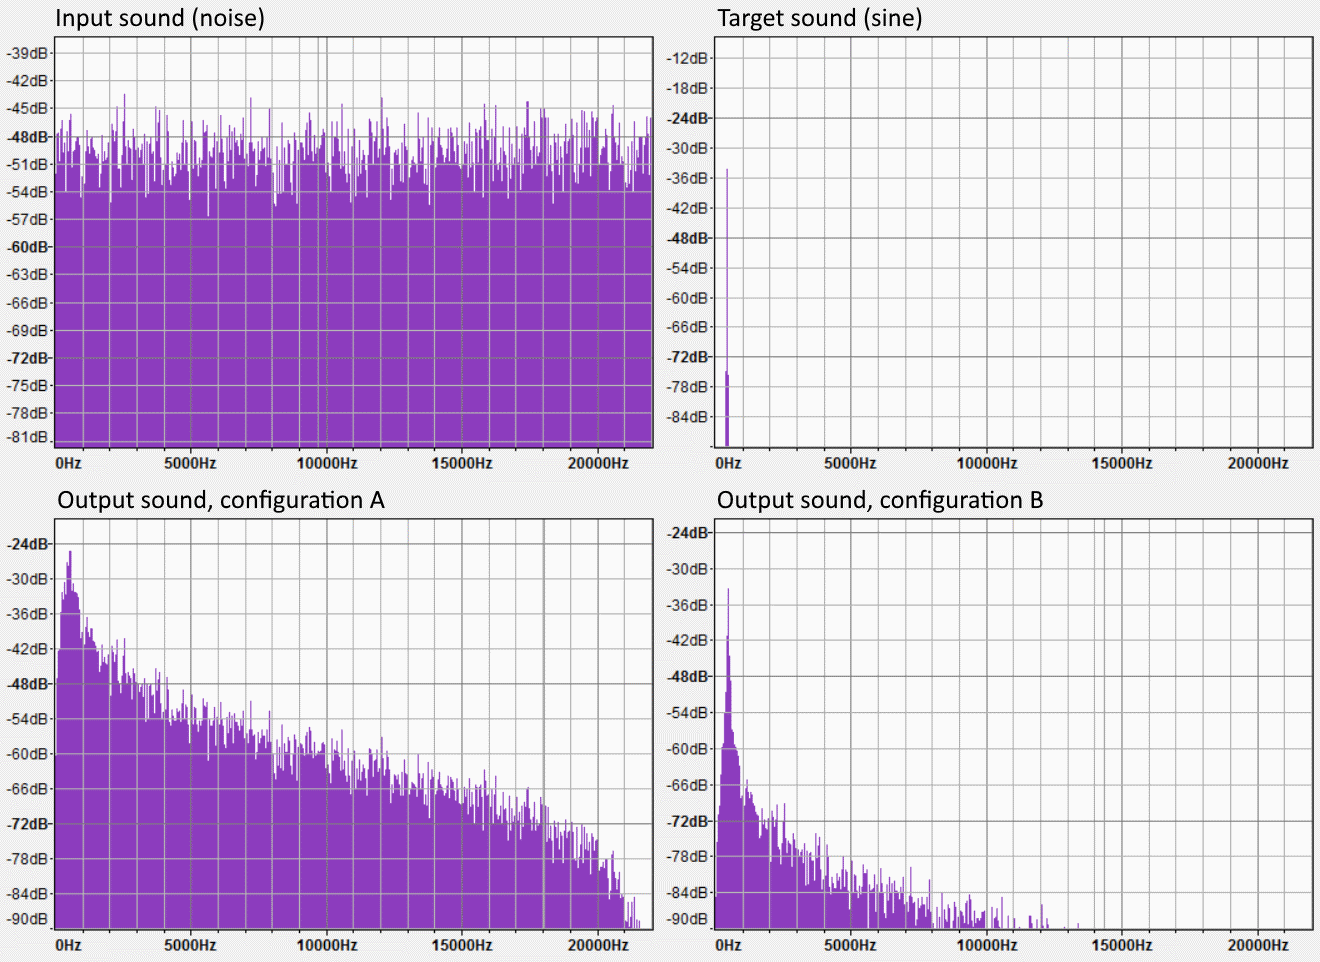
\includegraphics[width=0.99\textwidth]{exp4_spectrum_plot}
    \caption{Spectrum plots, created in Audacity® with hanning window of size 8192}
    \label{fig:exp4_spectrum_plot}
\end{figure}

The takeaway from this experiment is that
\begin{itemize}  
\item the collection of features used for similarity measures has a high impact on the result
\item bark bands are useful
\end{itemize}

\subsection{Analysis}

In this subsection, one of the runs in configuration B will be analyzed, to get a better understanding of how NEAT works in practice, and identify some things that can be improved upon.

In this experiment, the effect parameters do not have to be \textit{dynamically} controlled over time. A static value for each effect parameter (bandwidth, center frequency and post gain) would have been an optimal solution. However, in figure \ref{fig:exp4_typical_nn_evolution}, we see that the NEAT algorithm actually makes use all three input nodes (RMS, pitch and spectral centroid) as well as the constand bias node. The reason for this is that these three inputs do not vary much in the course of the sound, because the features of the sound that was analyzed (sine, 440 Hz) do not vary much over time (see figure \ref{fig:exp4_typical_nn_evolution}). Consequently, these three nodes act like a bias node with some noise.

Another interesting fact is that the number of hidden nodes tends to increase over time, even though these hidden nodes are not needed to get an optimal solution in this experiment. Any constant value can be sent to the output node without having to go through hidden nodes. This is another example of NEAT not finding the optimal solution. Having many hidden nodes hurts evolvability, because an arbitrary mutation on a complex individual is less likely to yield an improvement than the same operation on a simpler individual with fewer hidden nodes. Some form of regularization (punishment for more complex neural networks) could alleviate the problem. Another way to deal with this problem in experiments that do not require hidden nodes is setting AddNodeProbability to zero.

\begin{figure}[h]
    \centering
    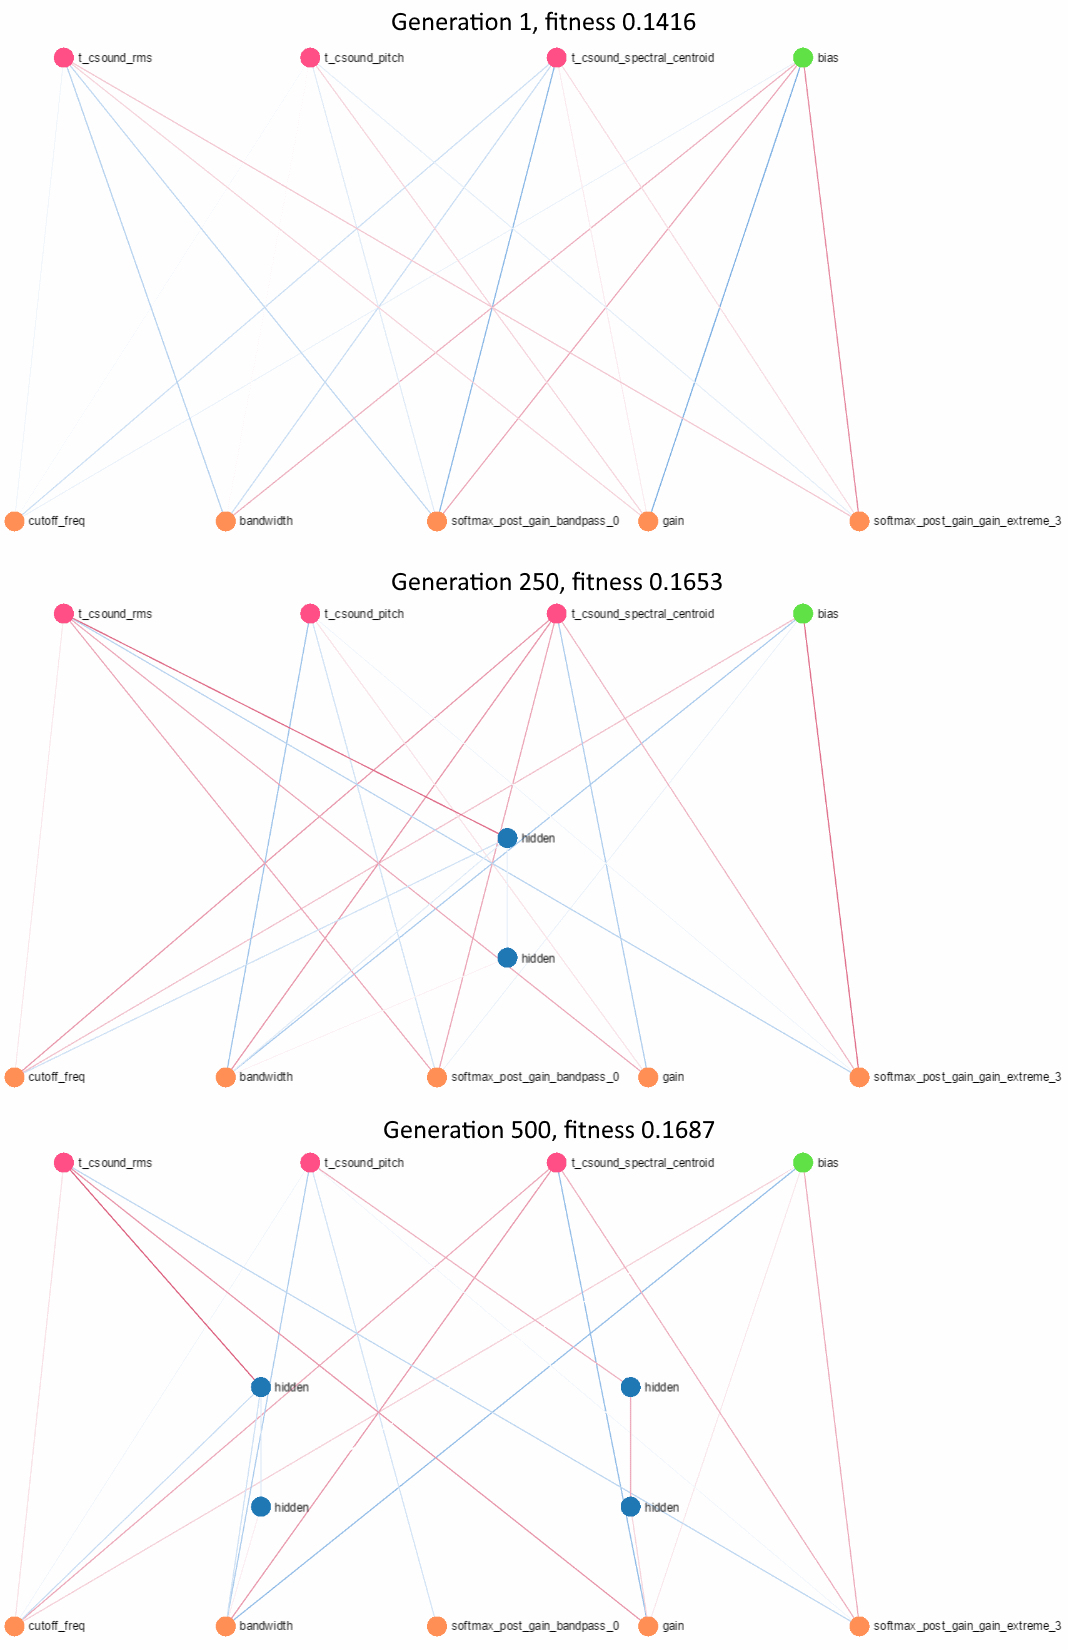
\includegraphics[width=0.9\textwidth]{exp4_typical_nn_evolution}
    \caption{Neural network visualizations}
    \label{fig:exp4_typical_nn_evolution}
\end{figure}

\begin{figure}[h]
    \centering
    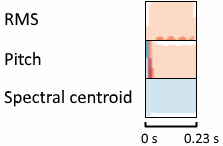
\includegraphics[width=0.3\textwidth]{exp4_neural_input}
    \caption{Neural inputs are almost constant}
    \label{fig:exp4_neural_input}
\end{figure}

\begin{figure}[h]
    \centering
    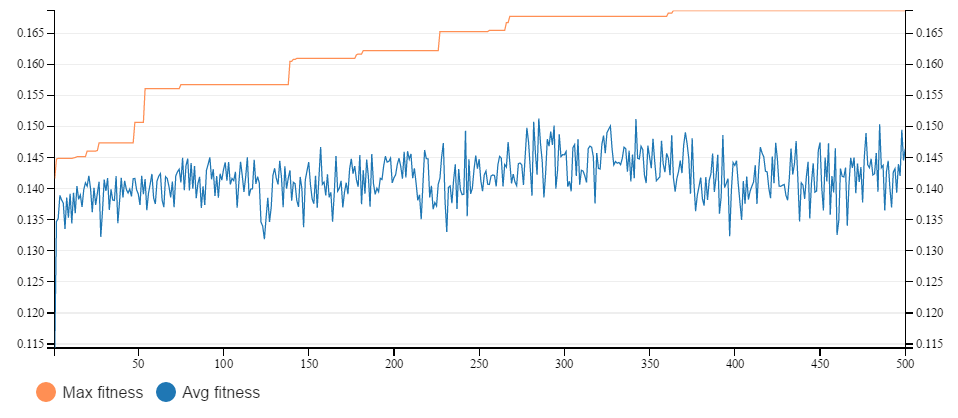
\includegraphics[width=0.99\textwidth]{exp4_fitness_plot}
    \caption{Fitness plot}
    \label{fig:exp4_fitness_plot}
\end{figure}

\begin{figure}[h]
    \centering
    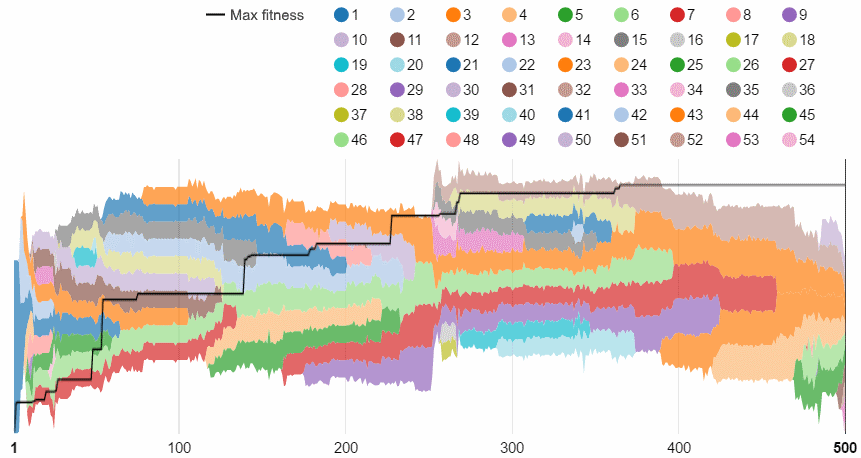
\includegraphics[width=0.99\textwidth]{exp4_species_plot}
    \caption{Species chart with max fitness overlay}
    \label{fig:exp4_species_plot}
\end{figure}

\iffalse
TODO Show species graph and discuss deaths and emerging species, correlate with fitness jumps.

regulated: between minspecies and maxspecies
each species at a given time has roughly the same amount of individuals
no obvious correlation between jumps in max fitness and the death of existing species or emergence of new species
competition happens only within species. species are given time to improve its structure before competition with the rest of the population occurs.
https://www.cs.cmu.edu/afs/cs/project/jair/pub/volume21/stanley04a-html/node3.html
\fi
